%pdflatex VFS.tex
%pdftoppm -png VFS.pdf output

\documentclass{standalone}


%\usepackage{graphicx}
\usepackage{tikz}
\usepackage{geometry}
\usetikzlibrary{automata, positioning, arrows, shapes.geometric,calc, shapes.multipart}
%\geometry{letterpaper}

%\newcommand{\specialcell}[2][b]{\begin{tabular}[#1]{@{}c@{}}#2\end{tabular}}

\begin{document}
	
	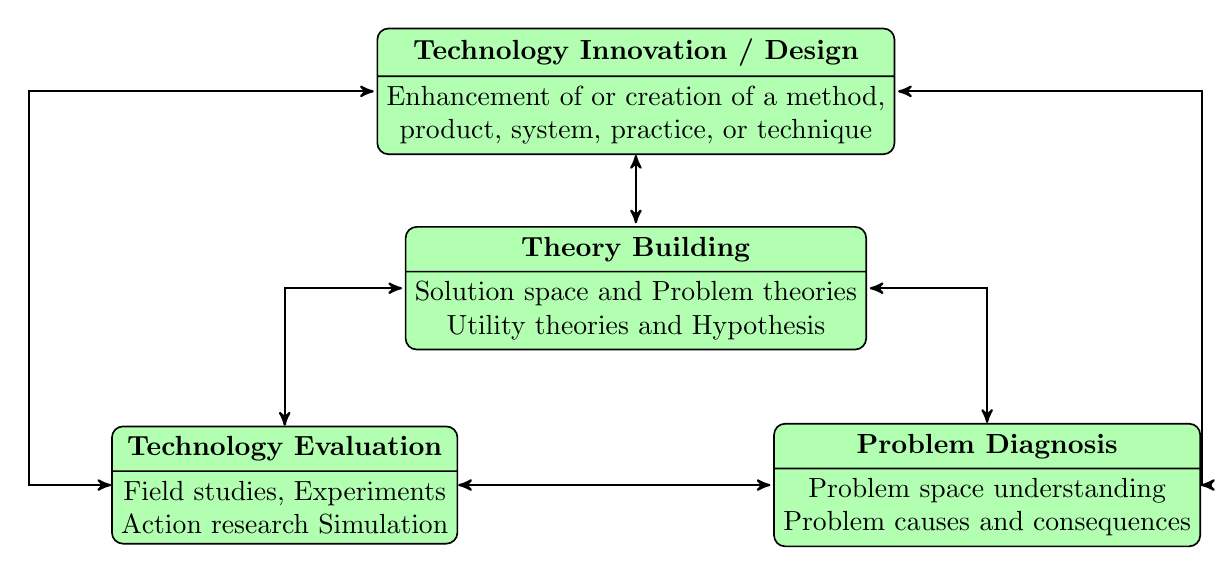
\begin{tikzpicture}[scale=0.50, ->, >=stealth', shorten >=1pt, node distance=6cm, semithick,
		every state/.style={rectangle, text centered, rounded corners, black, draw=black, fill=green!30, minimum width=2cm,minimum height=1.2cm,}]
		
		\node[state] (TechEval) [align=center, rectangle split, rectangle split parts=2] 
		{\textbf{Technology Evaluation} \nodepart{second} Field studies, Experiments \\ Action research Simulation};
		
		\node[state] (ProbDiag) [right=4cm of TechEval, align=center, rectangle split, rectangle split parts=2] 
		{\textbf{Problem Diagnosis} \nodepart{second} Problem space understanding \\ Problem causes and consequences};
		
		\node[state] (TechInnovDesg) [yshift=5cm, align=center, rectangle split, rectangle split parts=2] at ($(TechEval)!0.5!(ProbDiag)$)
		{\textbf{Technology Innovation / Design} \nodepart{second} Enhancement of or creation of a method, \\ product, system, practice, or technique};
		
		\node[state] (TheoryBld) [below of=TechInnovDesg, yshift=3.5cm, align=center, rectangle split, rectangle split parts=2]
		{\textbf{Theory Building} \nodepart{second} Solution space and Problem theories \\ Utility theories and Hypothesis};
		
		\draw[<->, thick] (TechInnovDesg.south) -- (TheoryBld.north);
		\draw[<->, thick] (TechEval.east) -- (ProbDiag.west);
		\draw[<->, thick] (TechEval.west) -| (-6.5,1.5) |- (TechInnovDesg.west);
		\draw[<->, thick] (TechEval.north) |- (TheoryBld.west);
		\draw[<->, thick] (ProbDiag.east) -| (23.3,1.5) |- (TechInnovDesg.east);
		\draw[<->, thick] (ProbDiag.north) |- (TheoryBld.east);
		
	\end{tikzpicture}

\end{document}

